%%%%%%%%%%%%%%%%%%%%%%%%%%%%%%%%%%%%%%%%%%%%%%%%%%%%%%%%%%%%%%%%%%%%%
%
% LaTeX Template
%
% This is a LaTeX document. LaTeX is a markup language for producing 
% documents. You will complete this document, compile it into a PDF 
% document, then upload it to the submission system. 
%
% To compile into a PDF on department machines:
% > pdflatex thisfile.tex
%
% If you do not have LaTeX, your options are:
% - Personal laptops (all common OS): http://www.latex-project.org/get/ 
%   + VSCode extension: https://marketplace.visualstudio.com/items?itemName=James-Yu.latex-workshop
% - Online Tool: https://www.overleaf.com/ - most LaTeX packages are pre-installed here (e.g., \usepackage{}).
%
% If you need help with LaTeX, please come to office hours.
% Or, there is help online:
% https://en.wikibooks.org/wiki/LaTeX
%
% Good luck!
%
%%%%%%%%%%%%%%%%%%%%%%%%%%%%%%%%%%%%%%%%%%%%%%%%%%%%%%%%%%%%%%%%%%%%%

\documentclass[11pt]{article}

\usepackage[english]{babel}
\usepackage[utf8]{inputenc}
\usepackage[colorlinks = true,
            linkcolor = blue,
            urlcolor  = blue]{hyperref}
\usepackage[a4paper,margin=1.5in]{geometry}
\usepackage{stackengine,graphicx}
\usepackage{fancyhdr}
\setlength{\headheight}{15pt}
\usepackage{microtype}
\usepackage{booktabs}
\usepackage{times}
\usepackage[shortlabels]{enumitem}
\setlist[enumerate]{topsep=0pt}
% a great python code format: https://github.com/olivierverdier/python-latex-highlighting
\usepackage{pythonhighlight}
\usepackage{amssymb}
\usepackage{multicol}
% setup for todo lists:
\usepackage{enumitem}
\newlist{todolist}{itemize}{2}
\setlist[todolist]{label=$\square$}
\usepackage{pifont}
\newcommand{\cmark}{\ding{51}}%
\newcommand{\done}{\rlap{$\square$}{\raisebox{2pt}{\large\hspace{1pt}\cmark}}%
\hspace{-2.5pt}}

\frenchspacing
\setlength{\parindent}{0cm} % Default is 15pt.
\setlength{\parskip}{0.3cm plus1mm minus1mm}

\pagestyle{fancy}
\fancyhf{}
\lhead{Project Writeup}
\rhead{CSCI 1290/1430}
\rfoot{\thepage}

\date{}

\title{\vspace{-1cm}Project 5 Writeup}


\begin{document}
\maketitle
\vspace{-3cm}
\thispagestyle{fancy}

\section*{Instructions}
\begin{itemize}
  \item Describe any interesting decisions you made during your project.
  \item Show and discuss your results.
  \item Feel free to include code snippets, images, and equations.
  \item Use as many pages as you need, but err on the short side 
  \item \textbf{Please make this document anonymous.}
\end{itemize}

I tried using Poisson and Laplacian blending, but they both looked really weird and I could not fix them, so I gave up on them and just used alpha blending.

Below are two images in 'homography,' 'translation,' 'rigid,' 'affine,' and 'cylindrical' in that order.

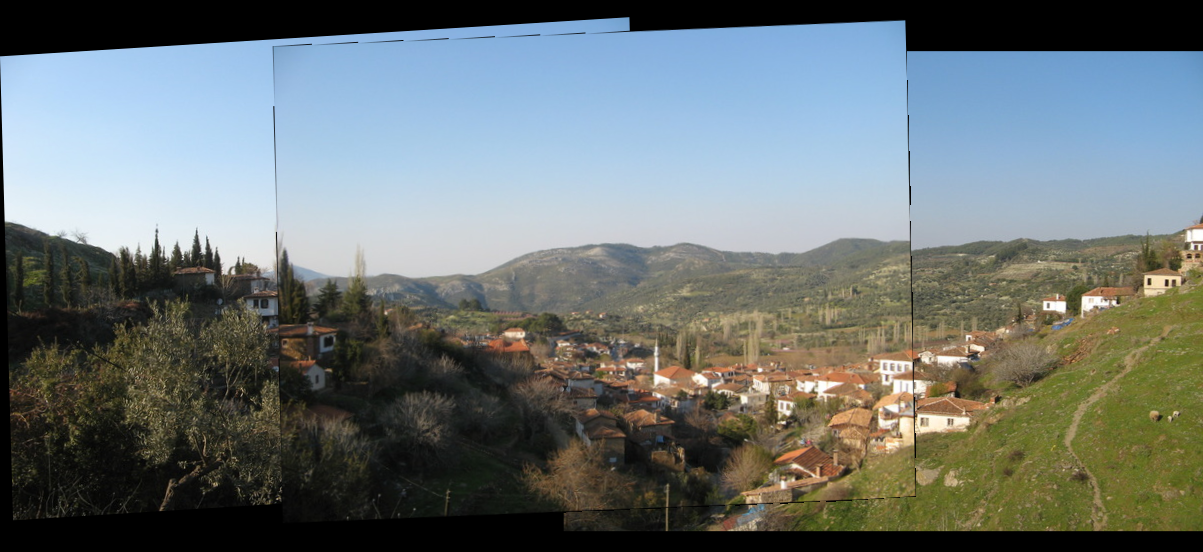
\includegraphics[width=\linewidth]{panorama_7_homography.png}
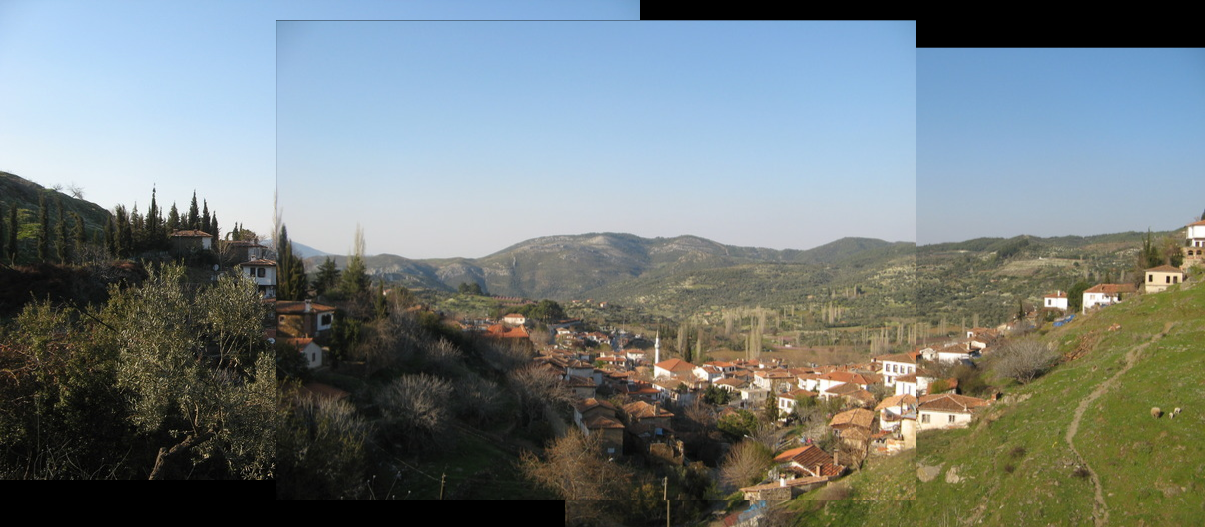
\includegraphics[width=\linewidth]{panorama_7_translation.png}
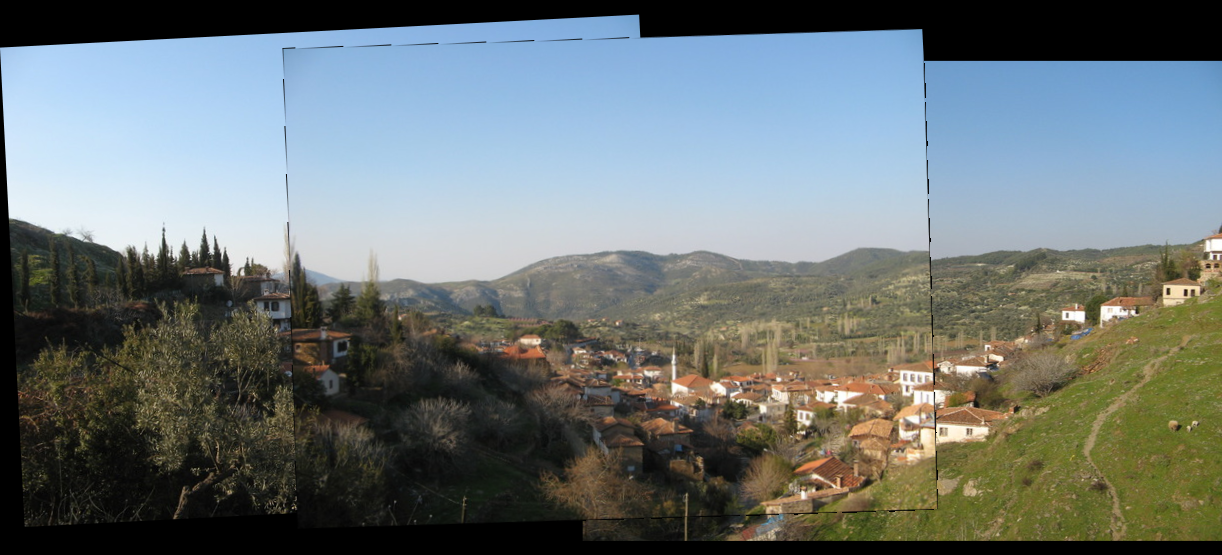
\includegraphics[width=\linewidth]{panorama_7_rigid.png}
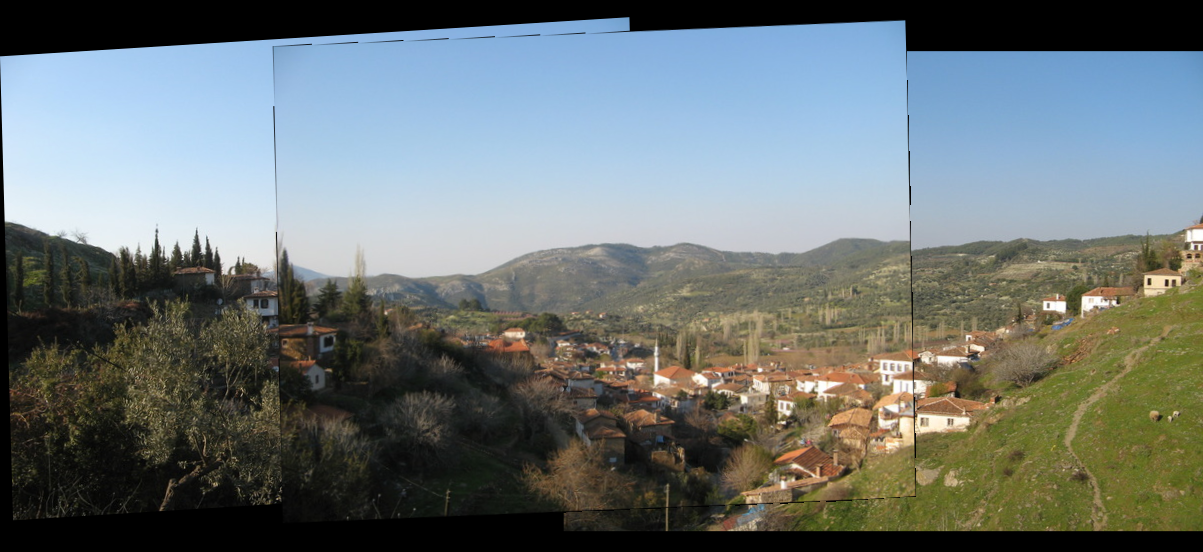
\includegraphics[width=\linewidth]{panorama_7_affine.png}
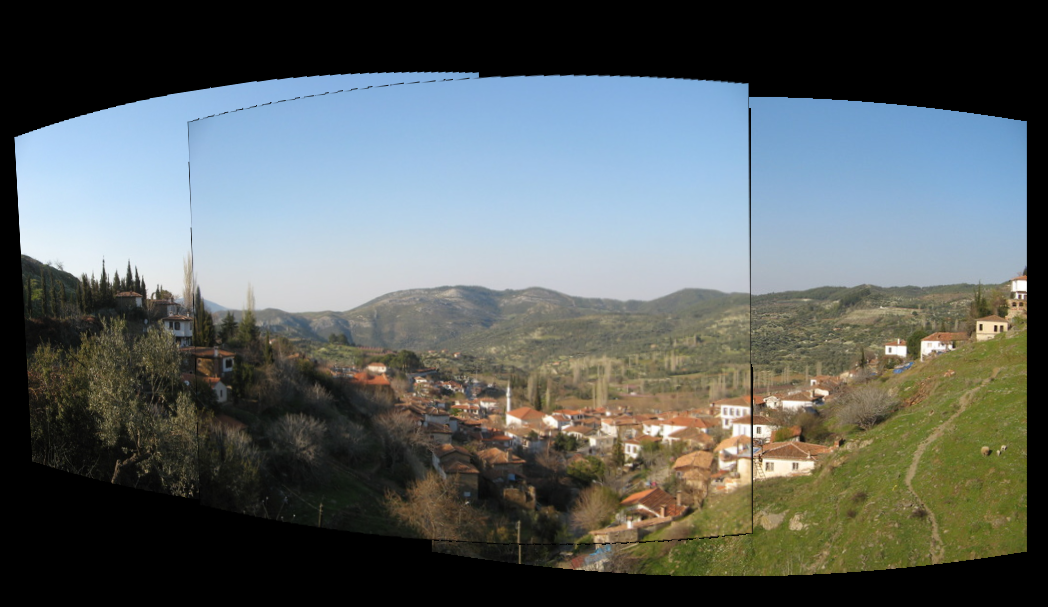
\includegraphics[width=\linewidth]{panorama_7_cylindrical.png}

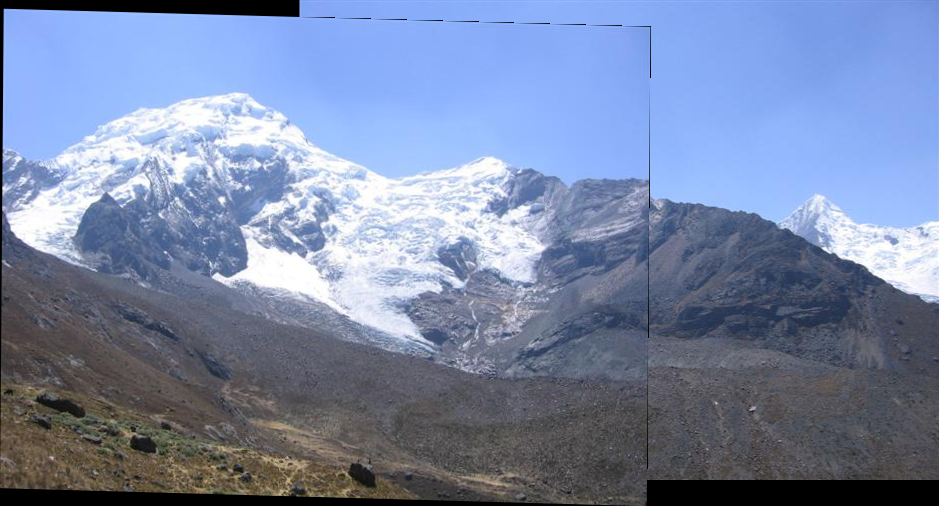
\includegraphics[width=\linewidth]{panorama_1_homography.png}
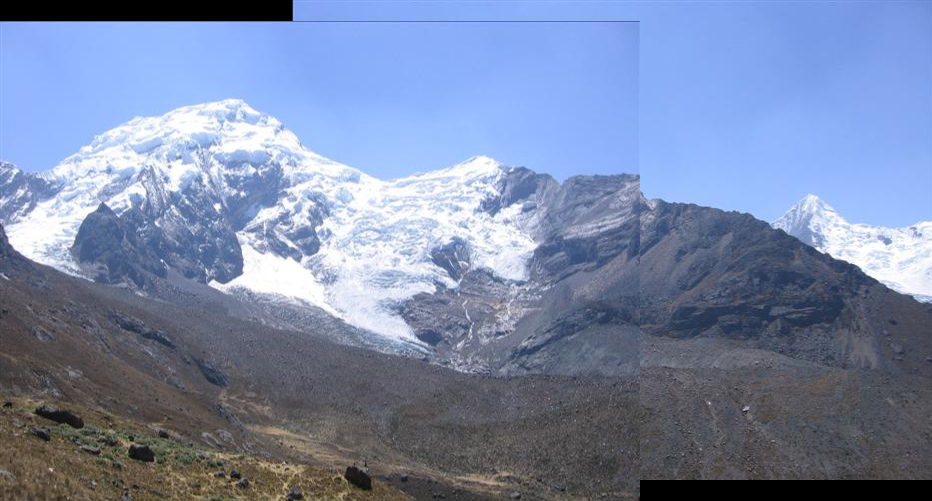
\includegraphics[width=\linewidth]{panorama_1_translation.png}
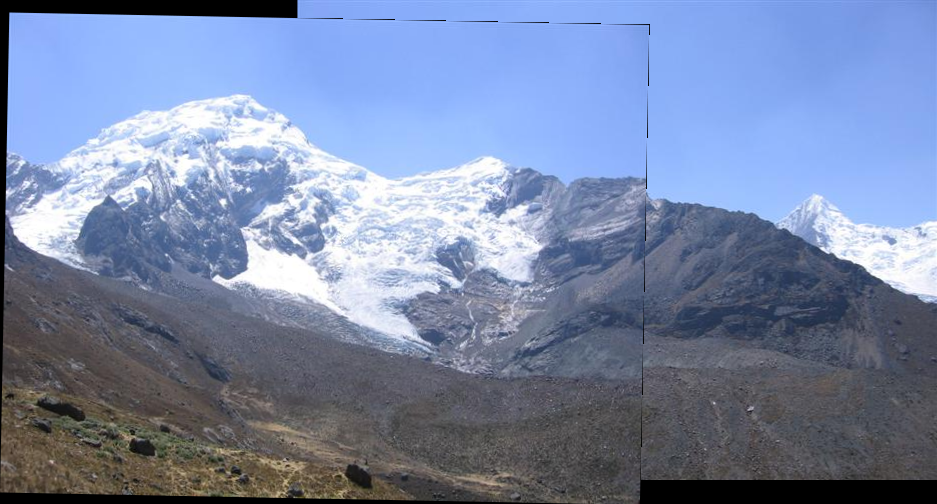
\includegraphics[width=\linewidth]{panorama_1_rigid.png}
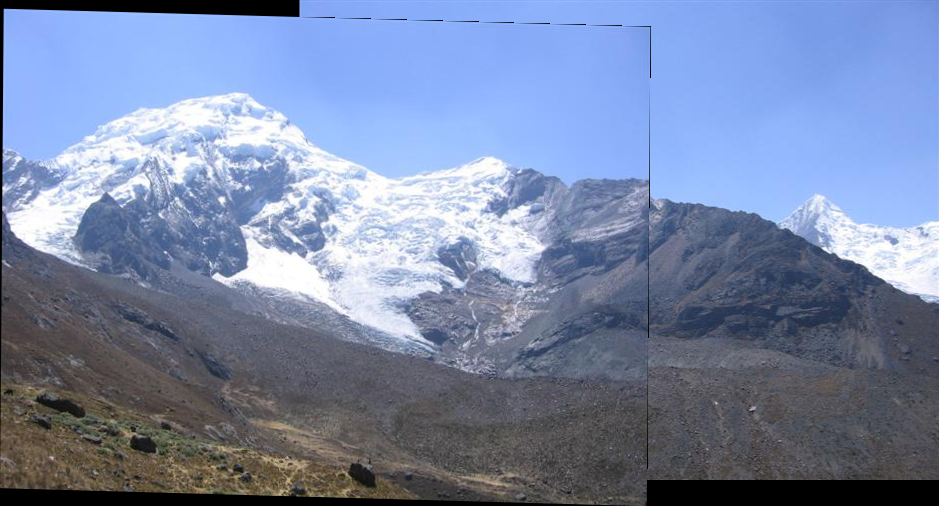
\includegraphics[width=\linewidth]{panorama_1_affine.png}
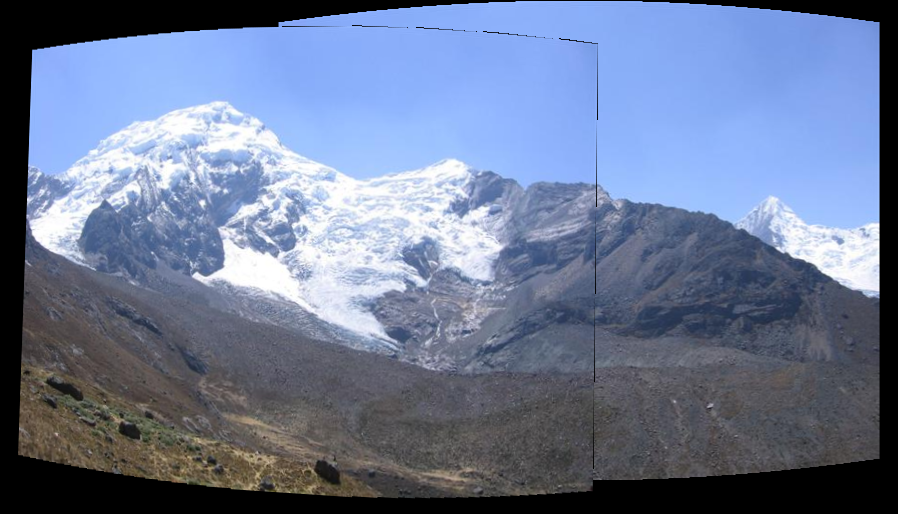
\includegraphics[width=\linewidth]{panorama_1_cylindrical.png}

\end{document}